\documentclass[a4paper]{article}
\usepackage[utf8]{inputenc}
\usepackage[T1]{fontenc}
\usepackage[brazil]{babel}
\usepackage{float}
\usepackage{graphicx}

\title{Etapa 5}
\author{Amilcar \and Marcelo Garlet Millani}
\date{}

\begin{document}

 \maketitle 
 
\section{Pacotes}
 
	\begin{figure}[H]
		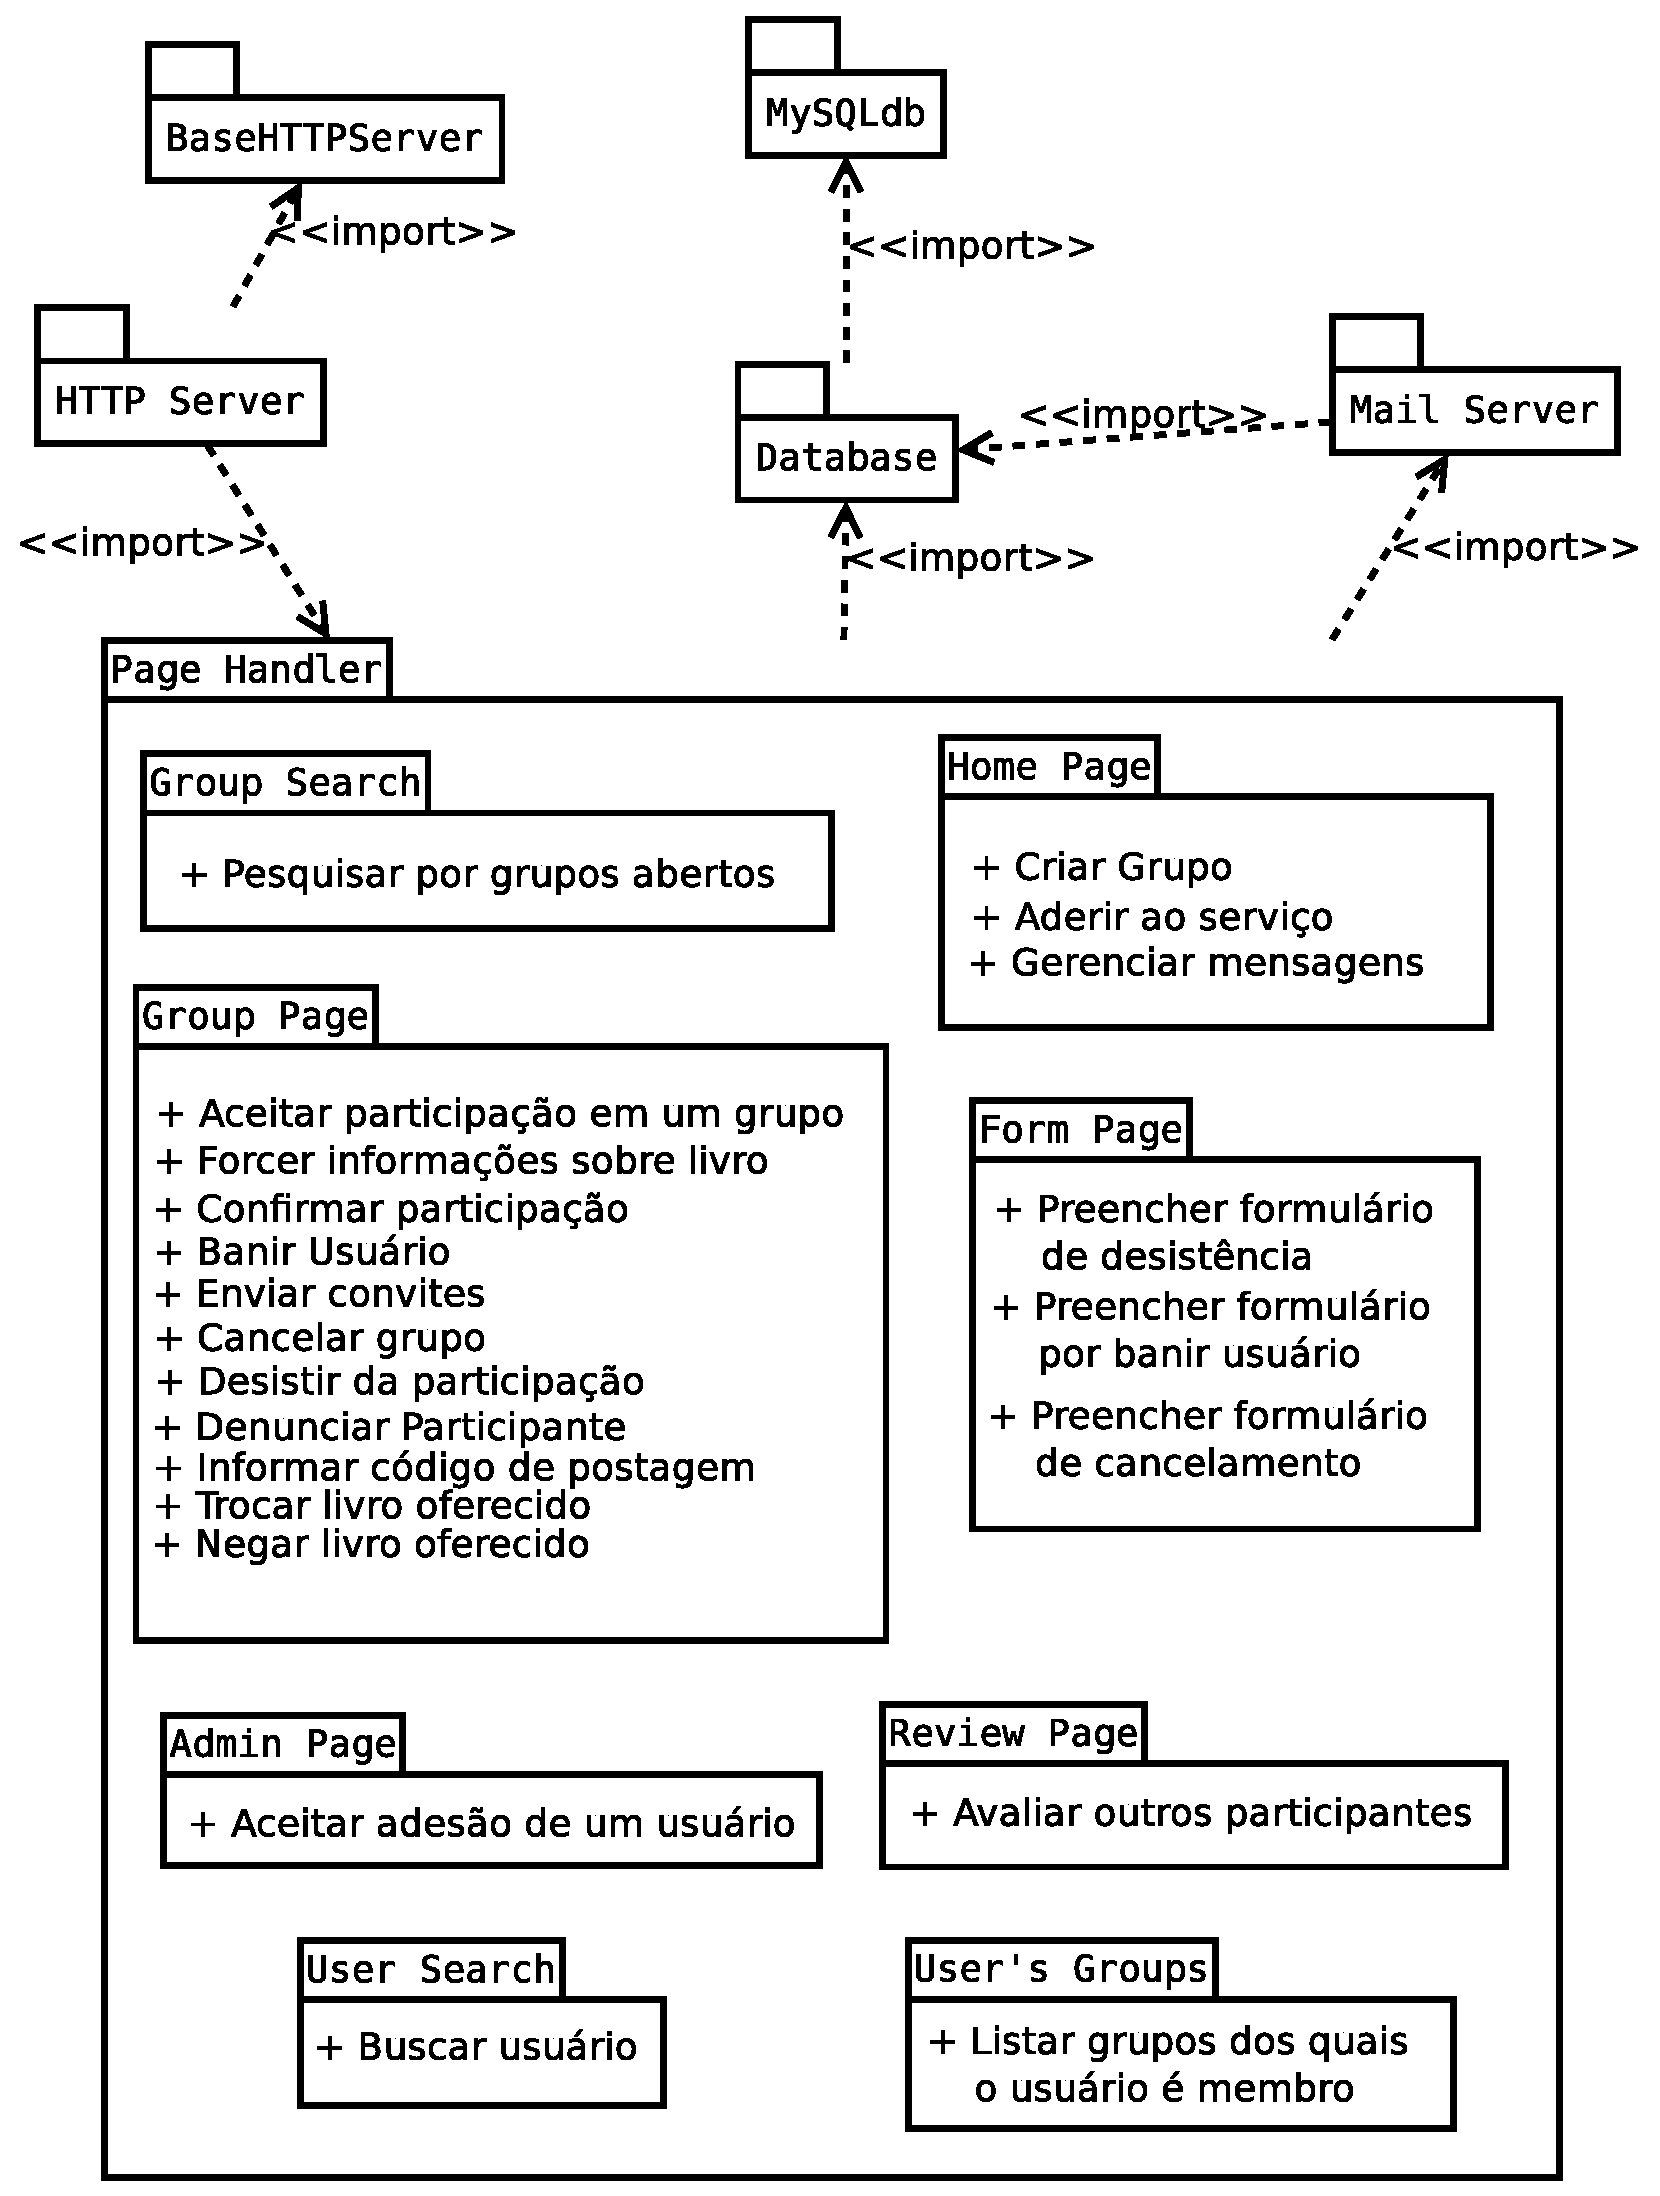
\includegraphics[totalheight=0.9\textheight]{pacotes.eps}
		\caption{Diagrama de Pacotes}
	\end{figure}
	
	Escolhemos uma arquitetura em camada para desenvolver o projeto. As camadas existentes são:
	\begin{description}
	 \item [Low-level Operations] Responsável por lidar com o acesso ao banco de dados para buscar e armazenar as informações.
	 \item [System Operations] Realiza as operações lógicas do sistema, isto é, implementa os casos de uso em si, mas delegando a concretização deles a camada de Low-level Operations e recebendo os pedidos da camada User Interface
	 \item [User Interface] Recebe diretamente os pedidos do usuário, sendo responsável por respeitar o protocolo HTTP e fazer com que a informação chegue ao usuário. Repassa os pedidos a camada System Operations, que deve processá-los e devolver os dados prontos para o usuário.
	\end{description}
	
	A razão dessa escolha se dá pelo fato de a aplicação ser Web. Nesse casos, é necessário que haja um servidor que recebe os pedidos do usuário e envia a resposta. Como queríamos concentrar as pesquisas no banco de dados em um único módulo de forma que algum problema com o SQL que ocorresse estaria melhor isolado. Com isso, ficávamos naturalmente com duas camadas: uma para interface e outra para o banco de dados. O mais lógico era criar uma outra camada onde a semântica das operações seria implementada, realizando assim os casos de uso.

	
\section{Componentes}
 
 \begin{figure}[H]
  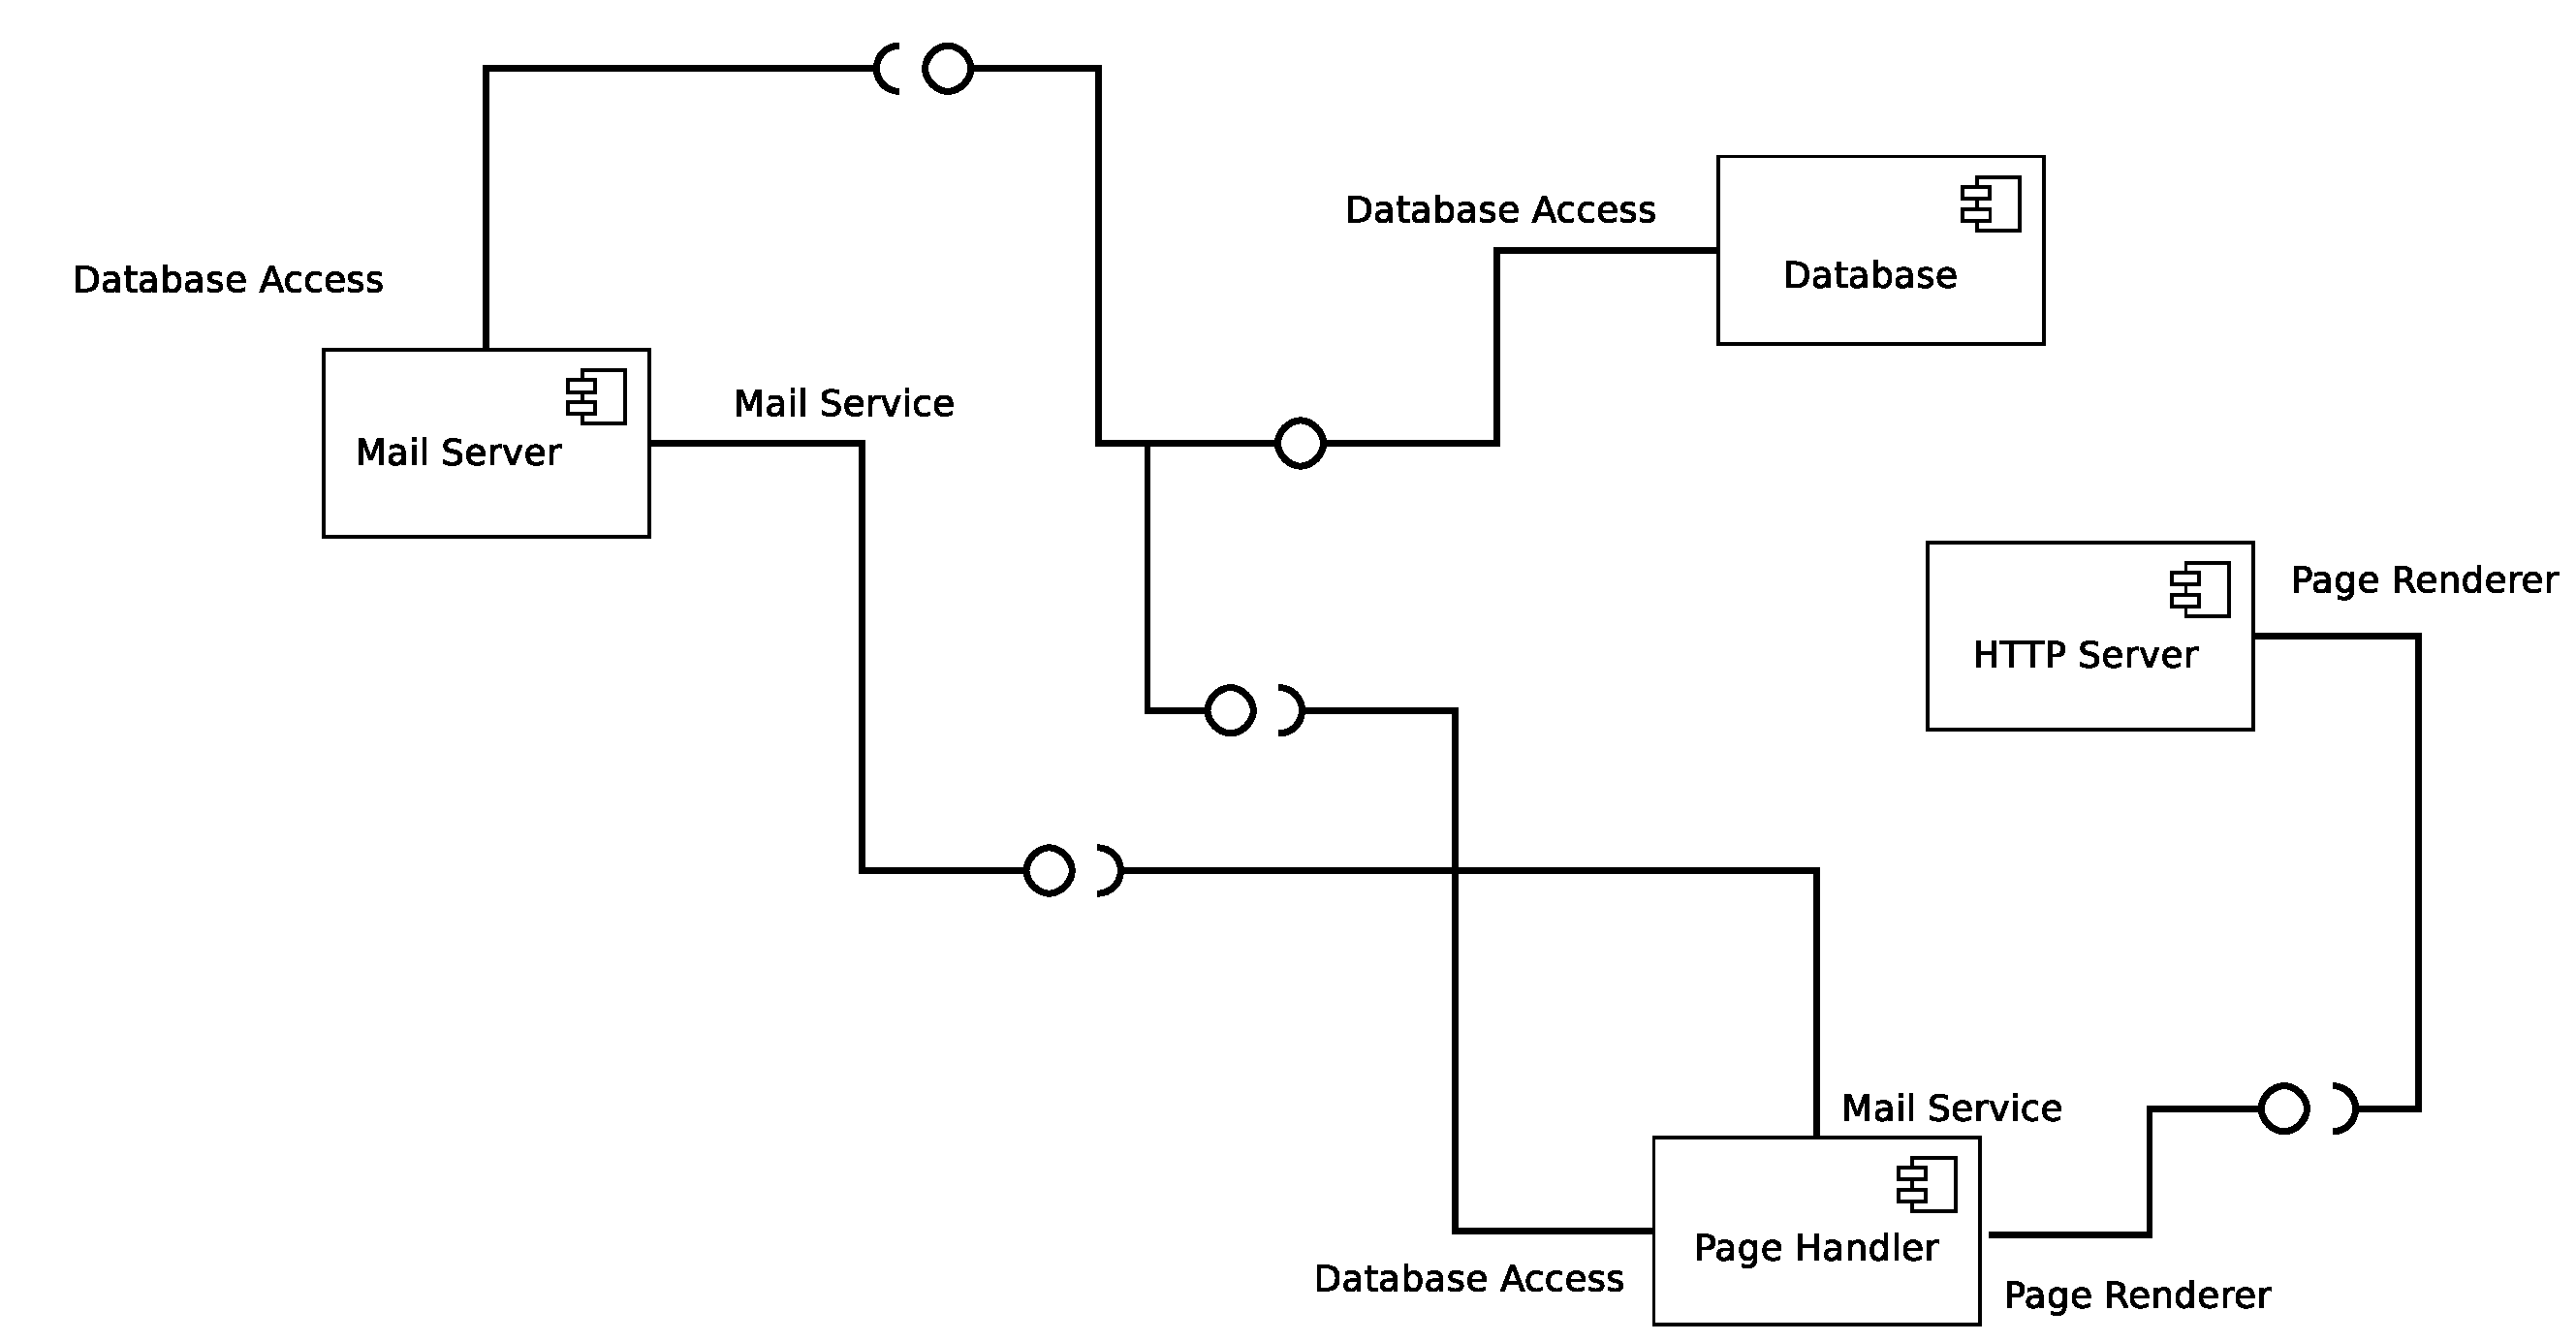
\includegraphics[angle=90,totalheight=0.9\textheight]{componentes.eps}
  \caption{Diagrama de Componentes}
 \end{figure}
 
\section{Modelo Entidade-Relacionamento}
 \begin{figure}[H]
  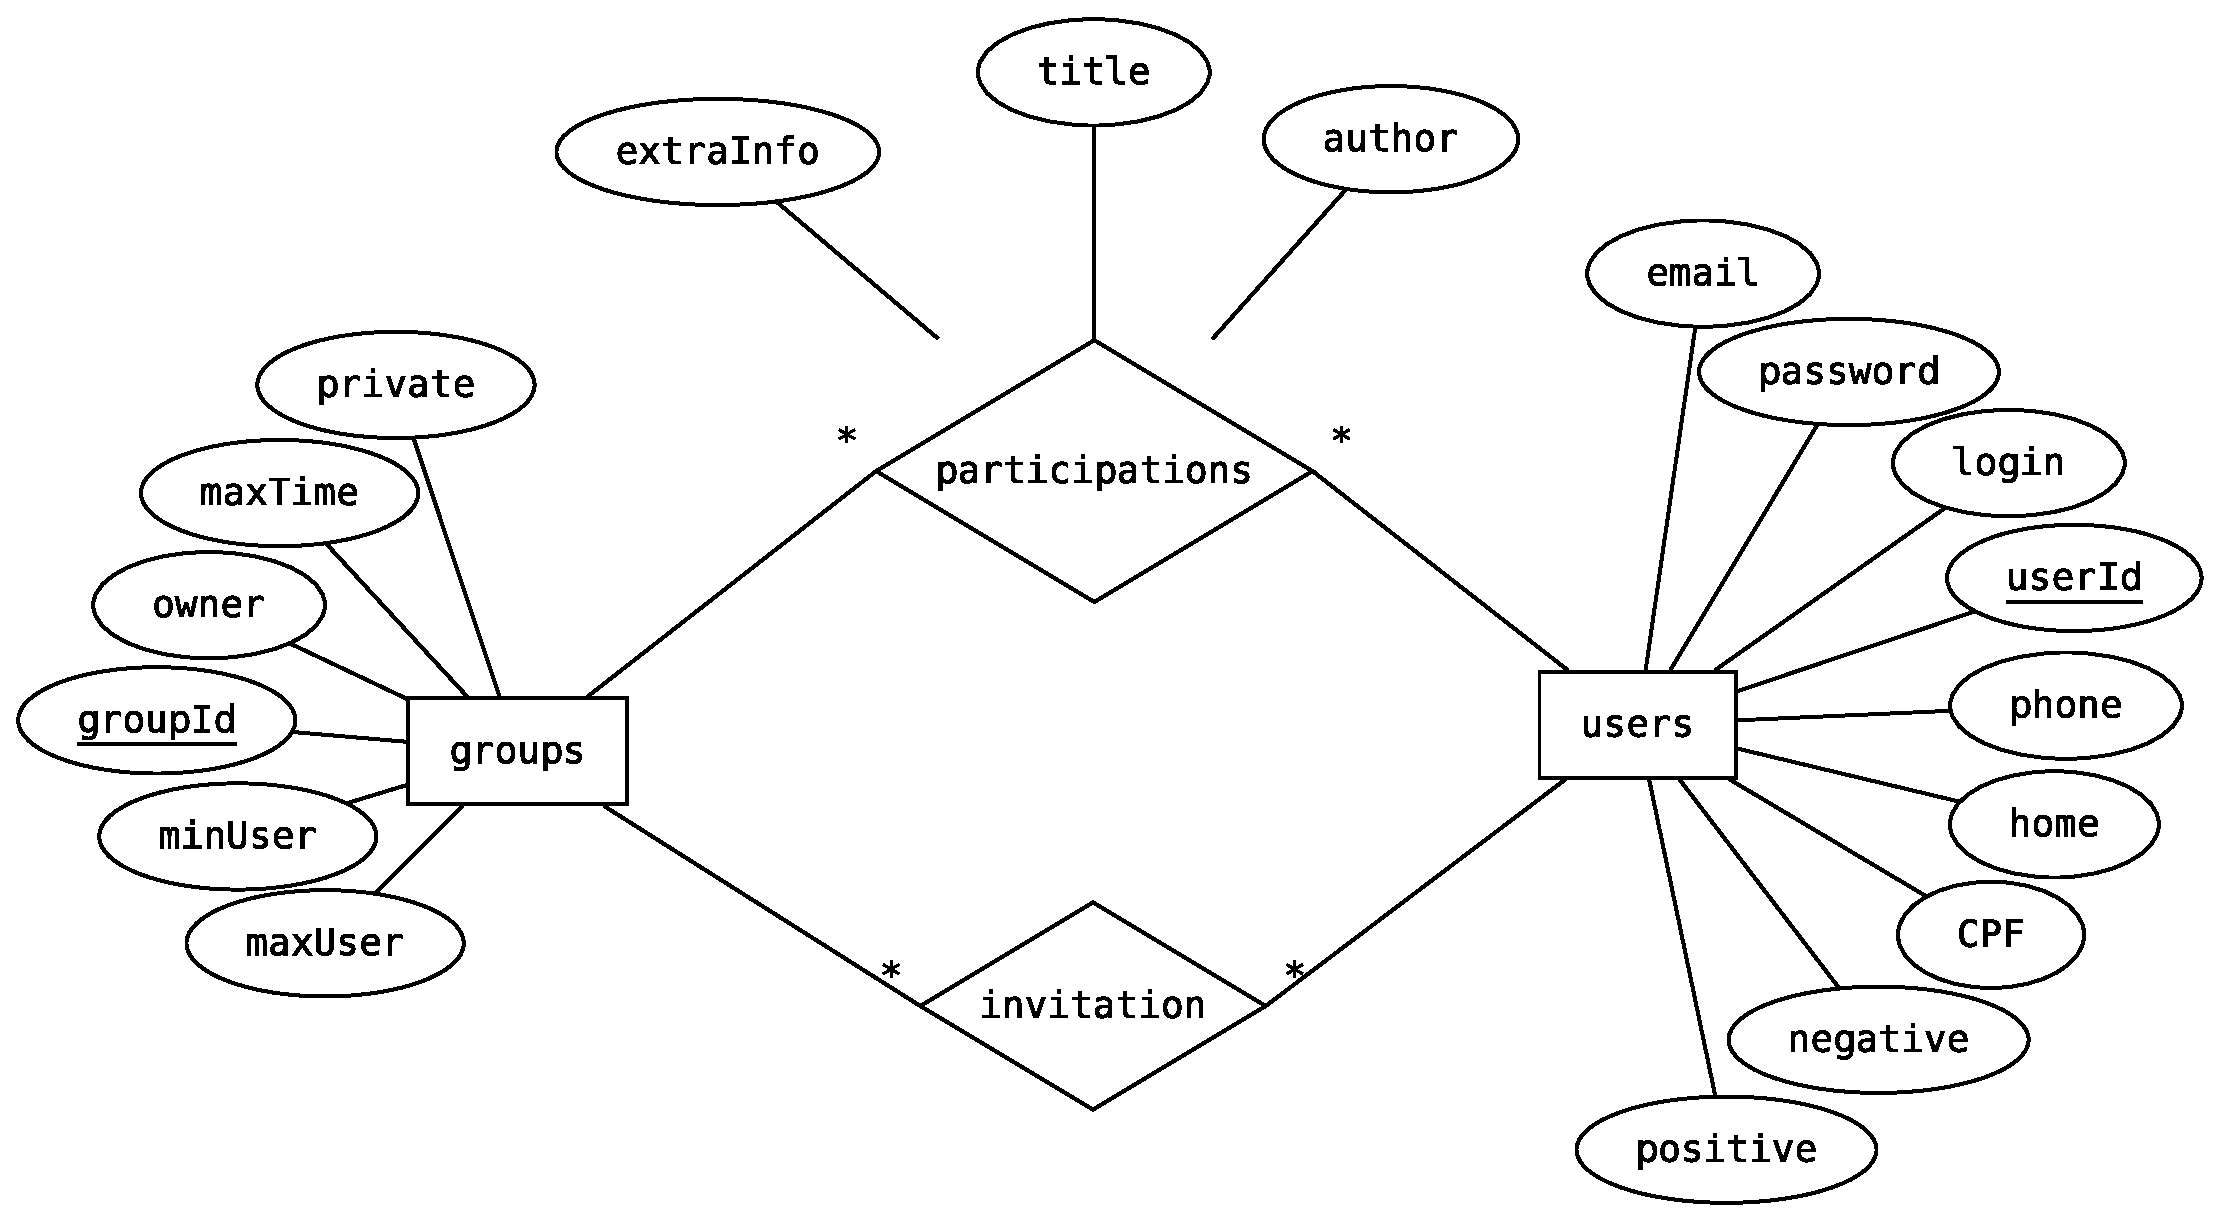
\includegraphics[angle=90,totalheight=0.8\textheight]{modeloER.eps}
  \caption{Modelo Entidade-Relacionamento}
 \end{figure}
 
\section{Casos de Uso}
 \begin{figure}[H]
  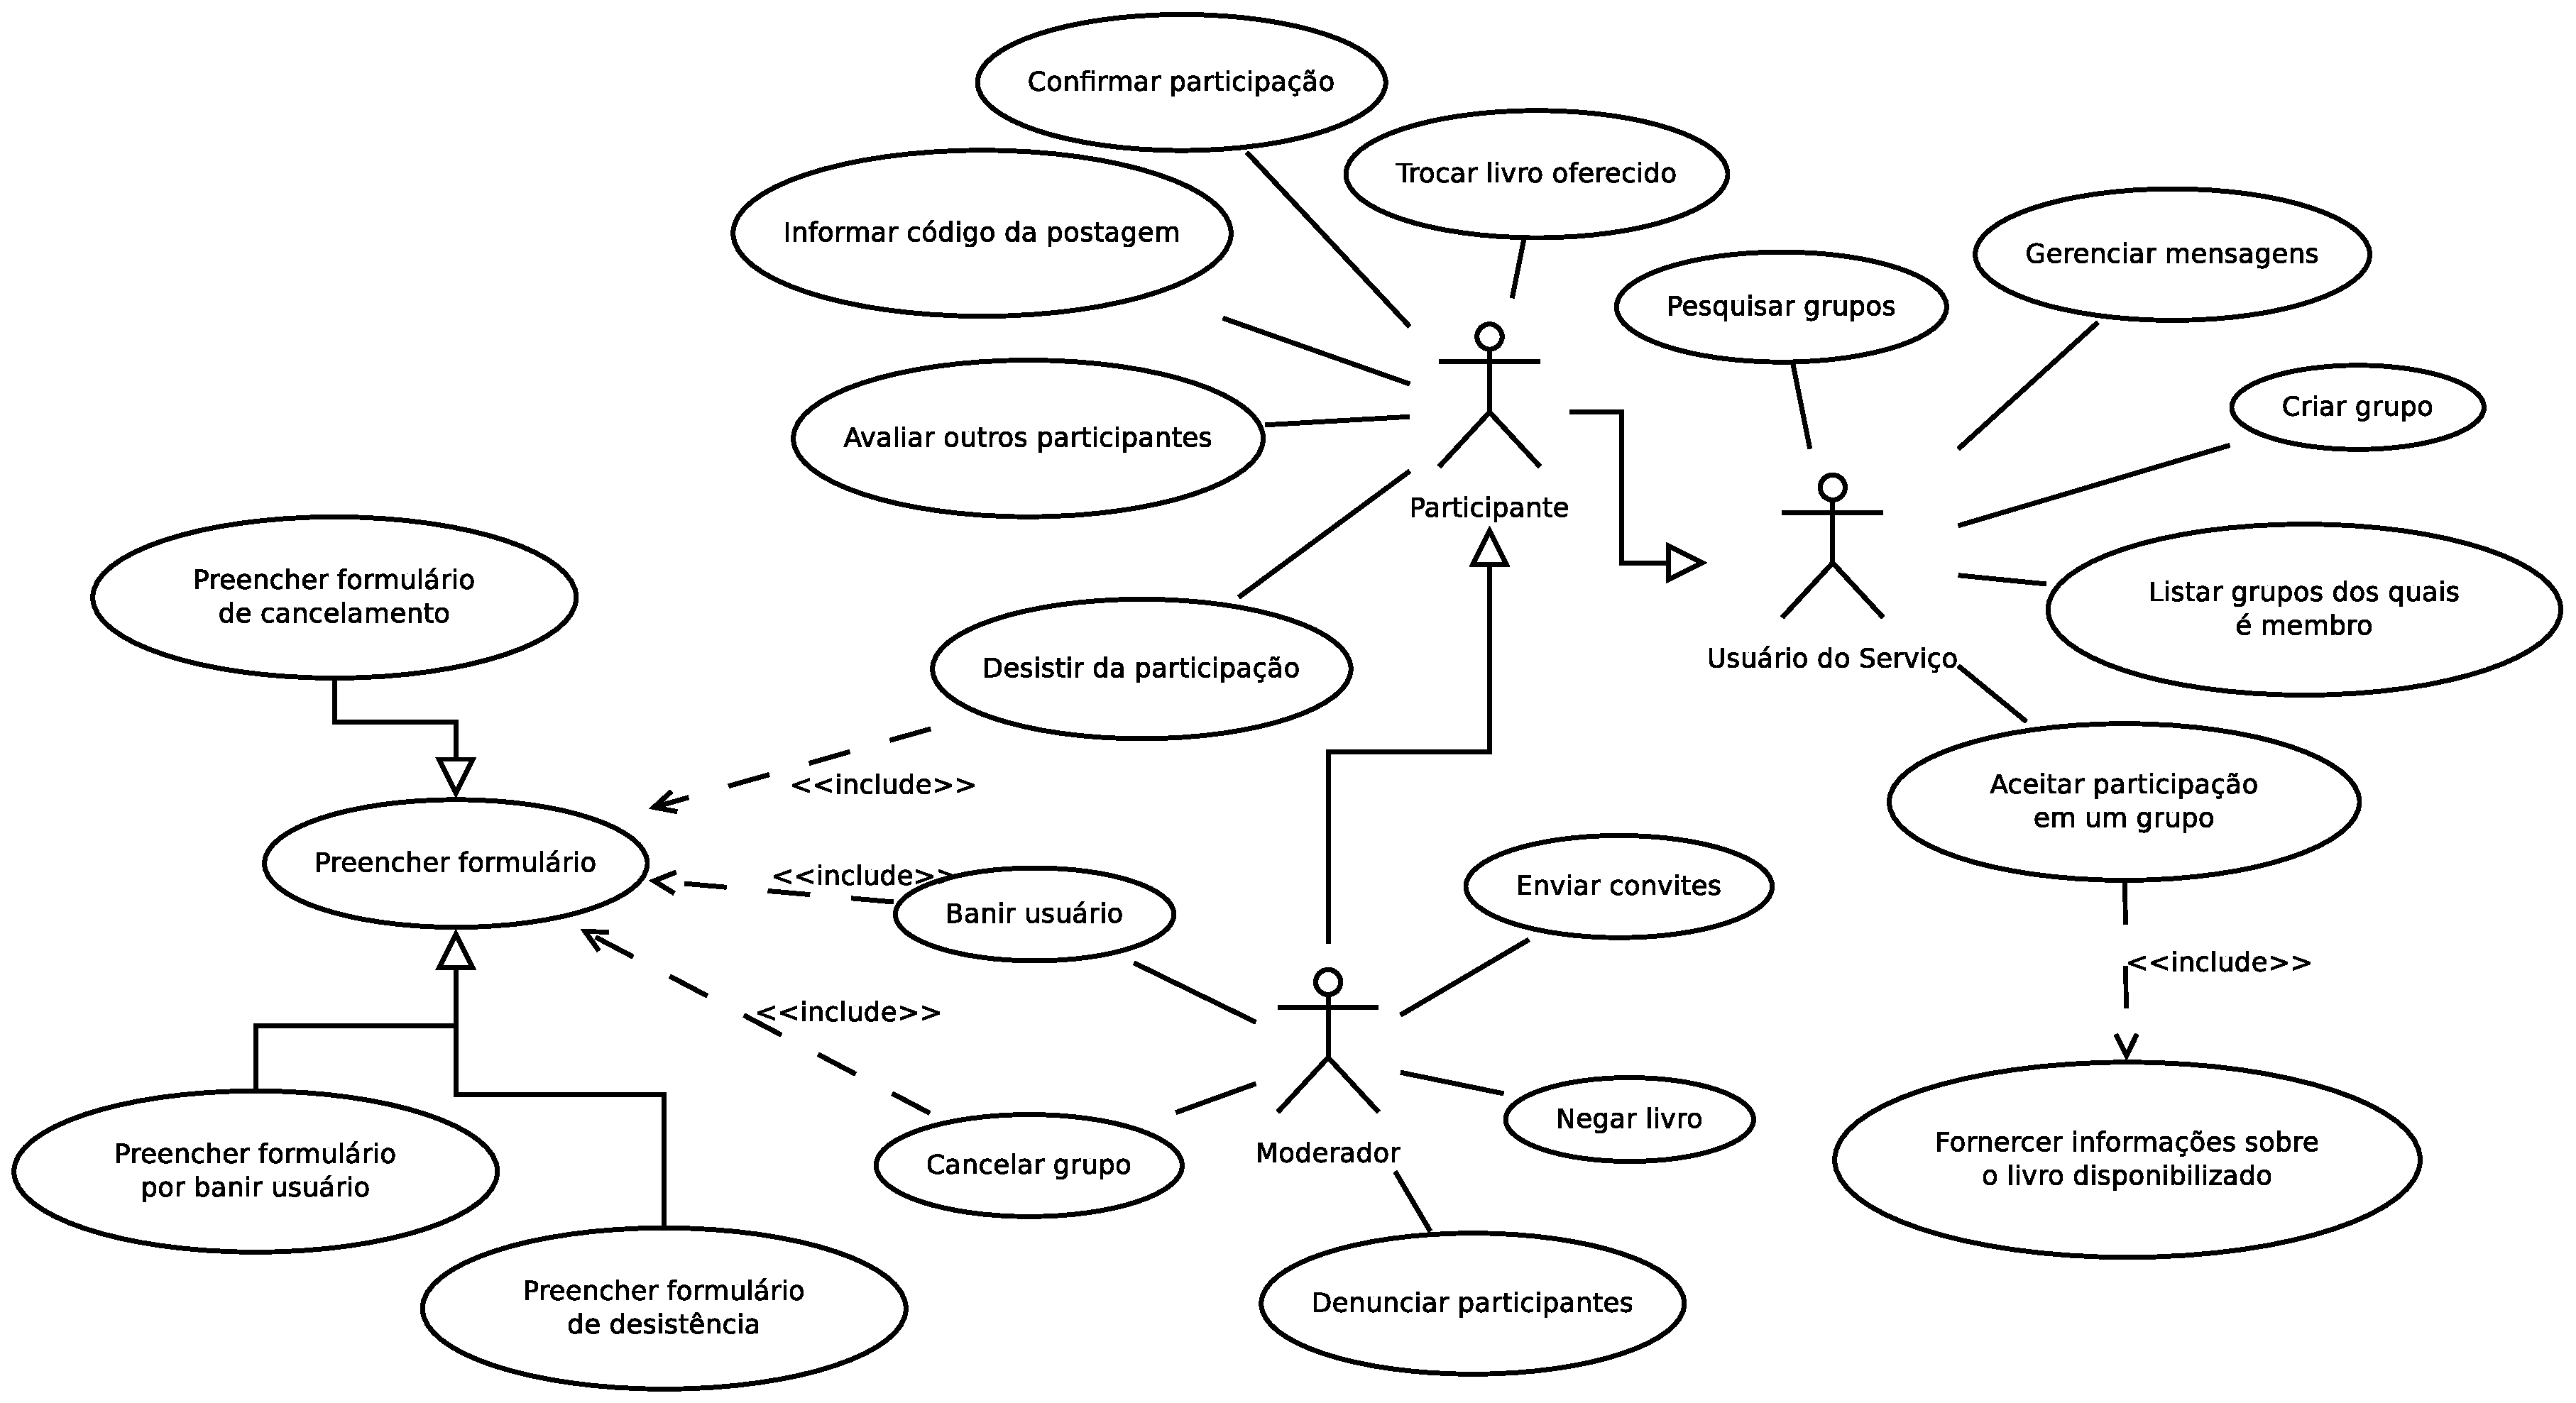
\includegraphics[angle=90,totalheight=0.9\textheight]{casosDeUso.eps}
  \caption{Diagrama de Casos de Uso}
 \end{figure}
 
\section{Sequência}
 \begin{figure}[H]
  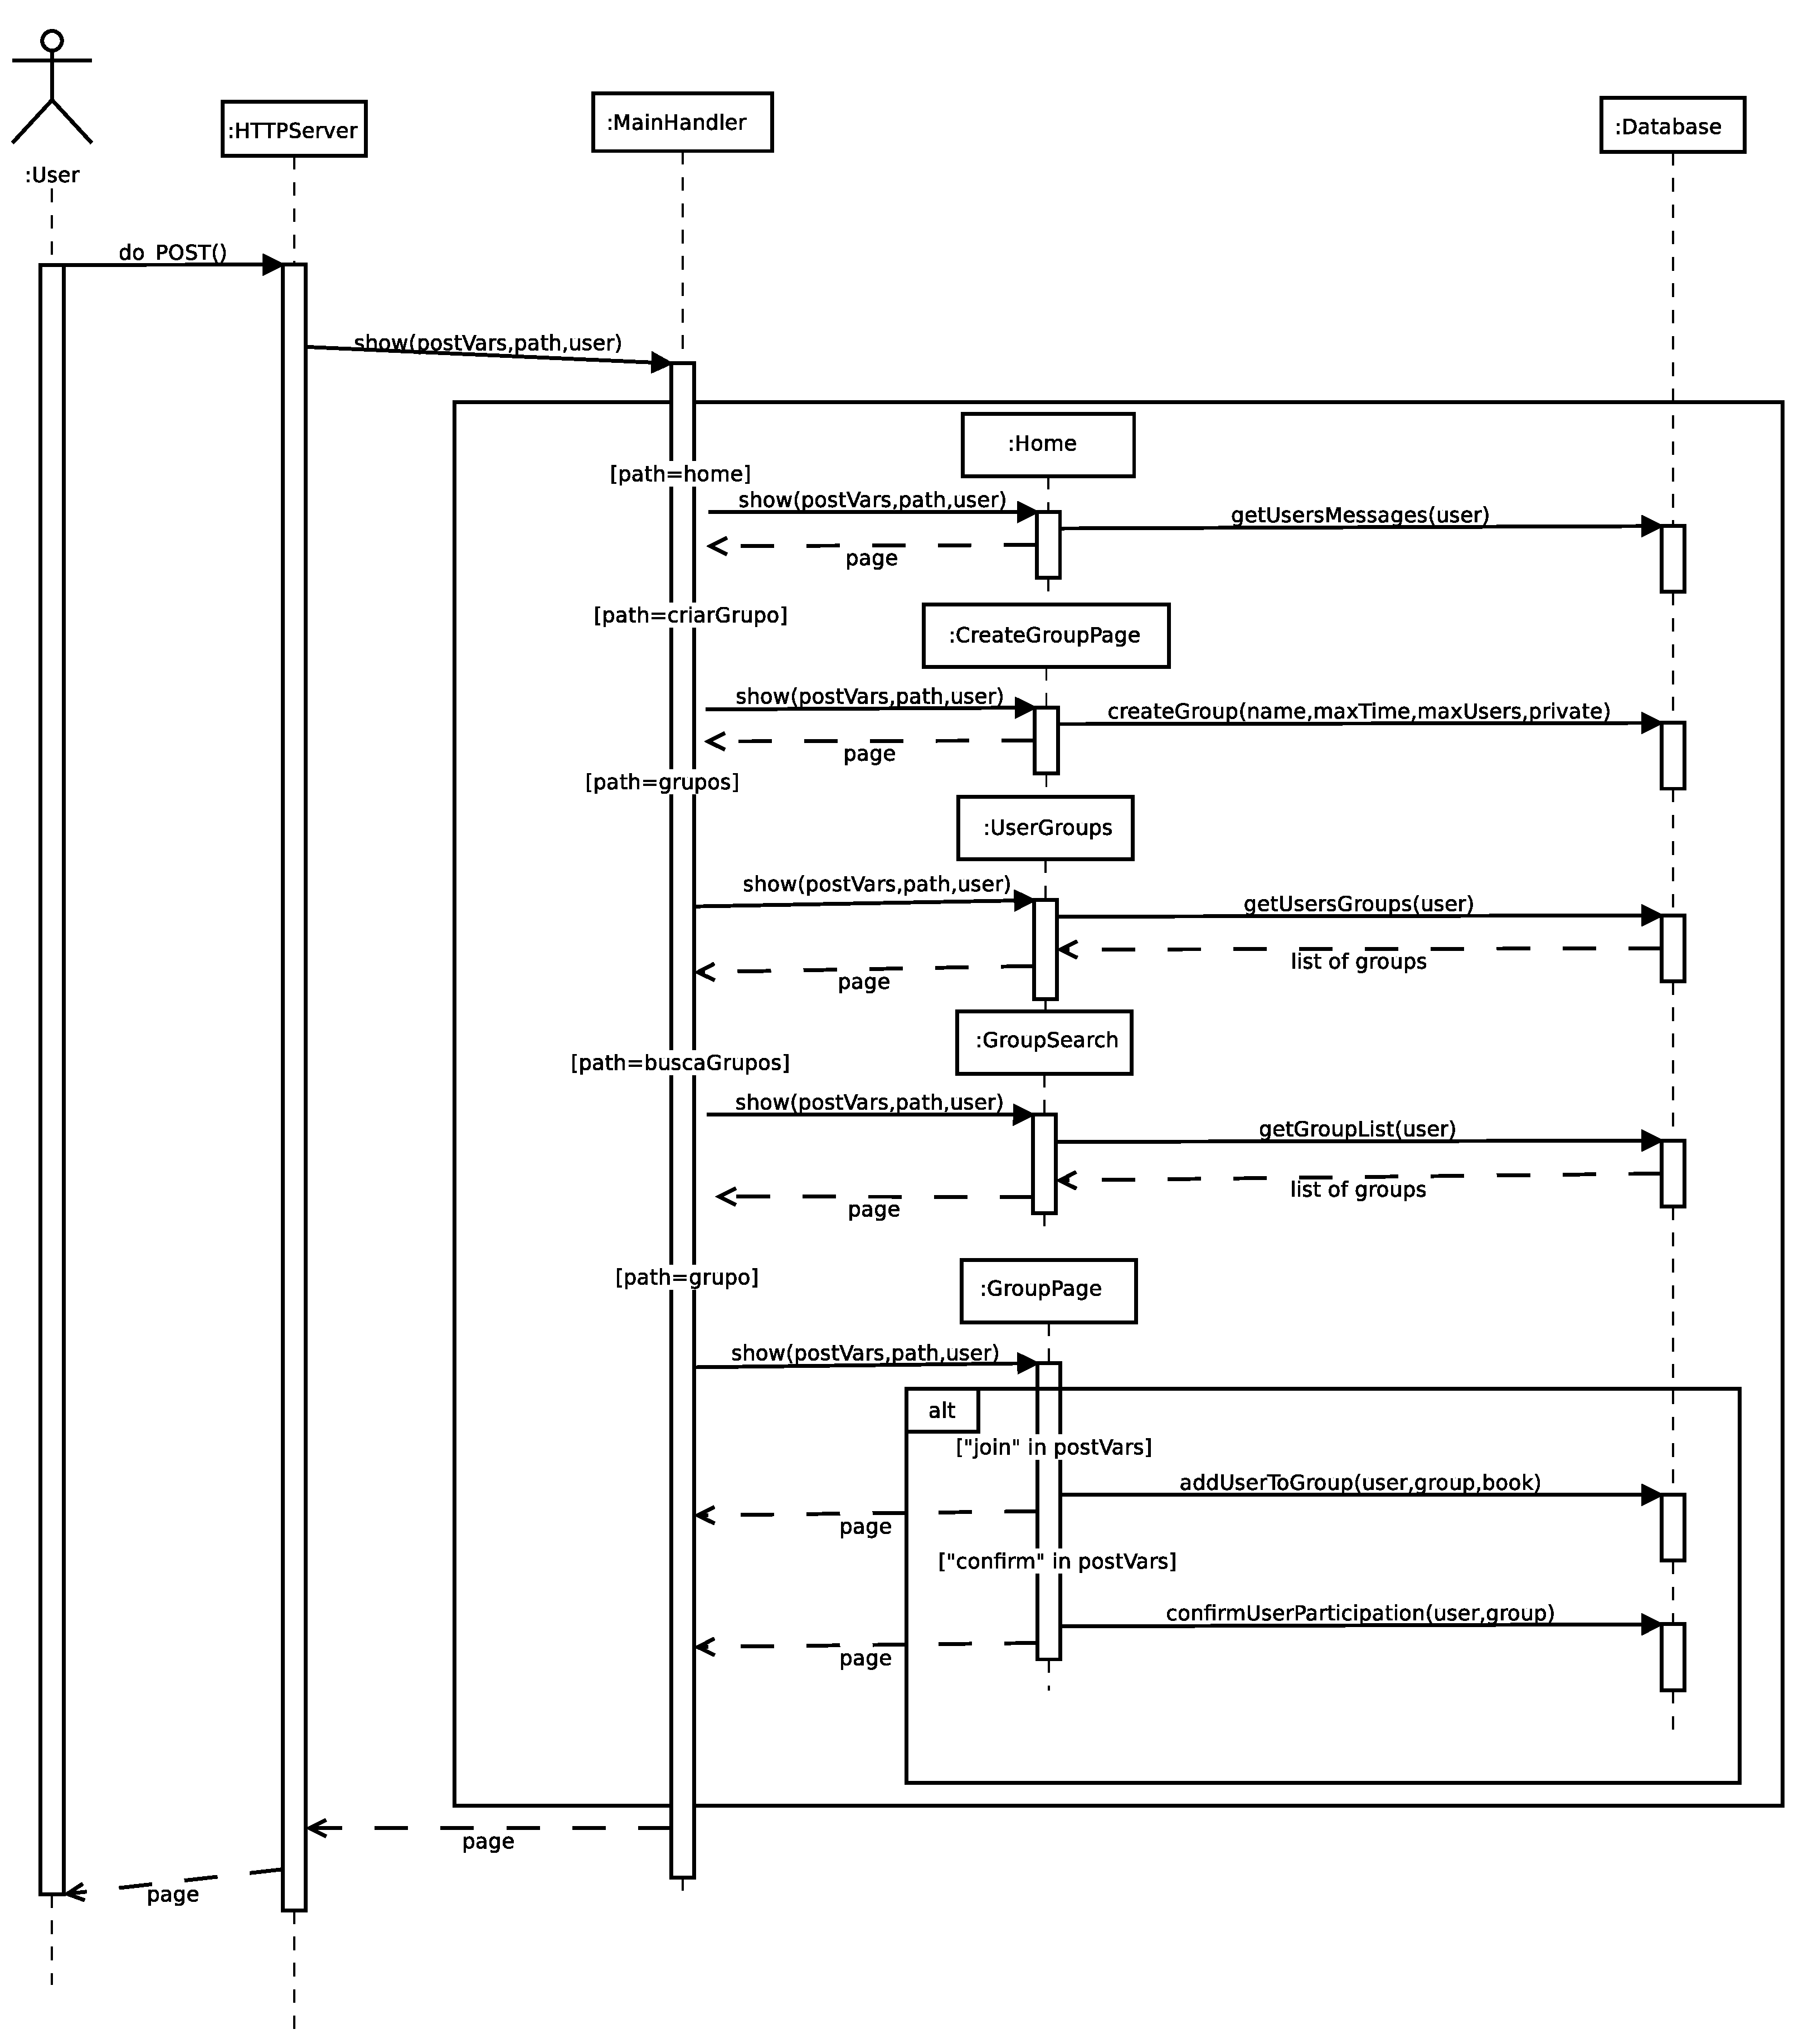
\includegraphics[width=\textwidth]{sequencia.eps}
  \caption{Diagrama de Sequência}
 \end{figure}
 
 \section{Classes}
 
 \begin{figure}[H]
  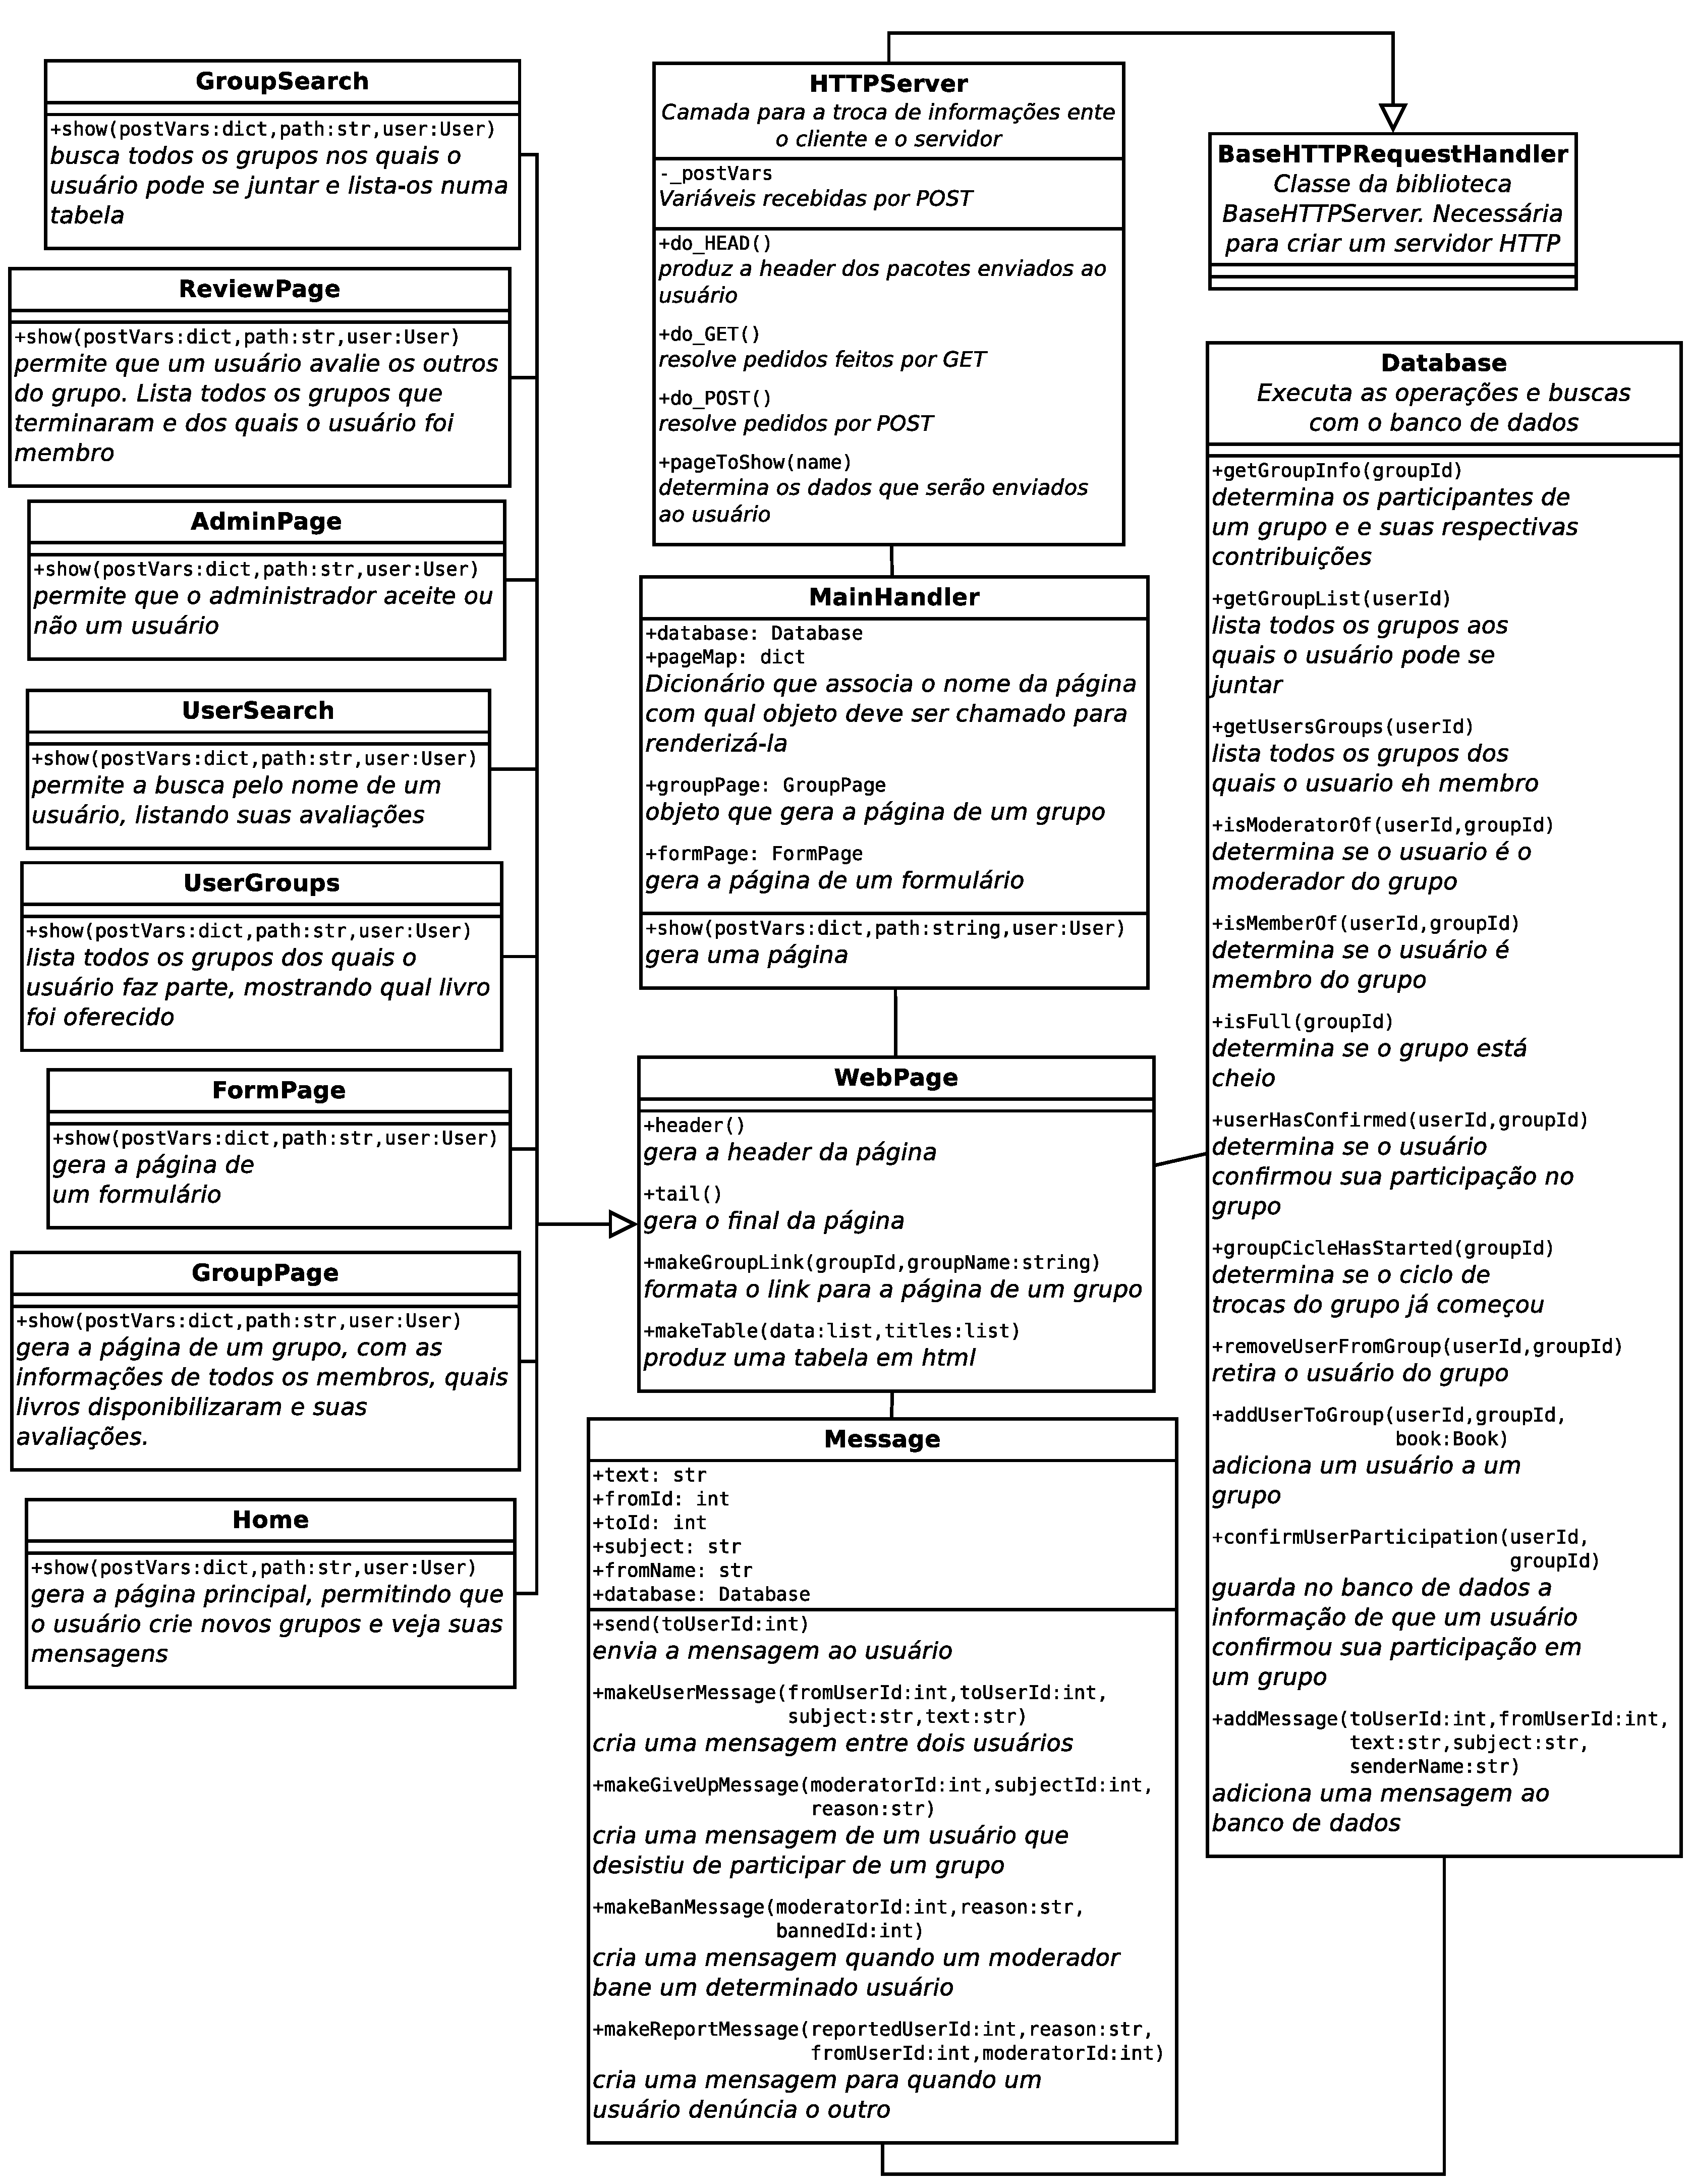
\includegraphics[width=\textwidth]{classes.eps}
  \caption{Diagrama de Classes}
 \end{figure}
 
 \subsection{HTTPServer}
 
	\begin{description}
		\item [Super classe] BaseHTTPRequestHandler (parte da biblioteca BaseHTTPServer)
		\item [Propósito] Gerenciar os pedidos do usuário em baixo nível, isto é, recebe as informações de GET e POST e envia os dados necessários para que o usuário receba a informação pedida.
	\end{description}
	
	\subsubsection{Atributos}
		\begin{description}
		 \item [\_postVars] Armazena as variáveis passadas por POST
			\begin{description}
			 \item [Visibilidade] Privado
			\end{description}

		\end{description}

	
	\subsubsection{Métodos}
		\begin{description}
		 \item [do\_Head] produz a header dos pacotes enviados ao usuário
			\begin{description}
			 \item [visibilidade] Público
			 \item [retorno] NoneType
			\end{description}
			
			\item [do\_GET] resolve pedidos do tipo GET
			\begin{description}
			 \item [visibilidade] Público
			 \item [retorno] NoneType
			\end{description}
			
			\item [do\_POST] resolve pedidos do tipo POST. Atualiza postVars
			\begin{description}
			 \item [visibilidade] Público
			 \item [retorno] NoneType
			\end{description}
			
			\item [pageToShow] determina qual página foi pedida pelo usuário
			\begin{description}
			 \item [visibilidade] Privado
			 \item [entrada] \mbox{}
				\begin{description}
				 \item [name : str] Nome do conteúdo pedido
				\end{description}
				
			 \item [retorno : (str,str)] conteúdo da página e tipo do conteúdo
			\end{description}
		\end{description}
		
	\subsection{Database}
	
	\begin{description}
		\item [Propósito] Centralizar as pesquisas no banco de dados de forma que conhecimento deste seja apenas necessário dentro da classe.
	\end{description}
	
	\subsubsection{Atributos}
		\begin{description}
		 \item [host] Onde está o banco de dados
			\begin{description}
			 \item [Visibilidade] Público
			\end{description}
		
		\item [user] Nome de usuário para acessar o banco de dados
			\begin{description}
			 \item [Visibilidade] Público
			\end{description}
			
		\item [passwd] Senha para acessar o banco de dados
			\begin{description}
			 \item [Visibilidade] Público
			\end{description}
			
		\item [db] Nome da Database
			\begin{description}
			 \item [Visibilidade] Público
			\end{description}

		\end{description}

	
	\subsubsection{Métodos}
		\begin{description} % métodos
		 \item [getGroupInfo] determina as informações do grupo sobre os livros oferecidos, número de participantes e avaliações dos membros
			\begin{description} % propriedades
			 \item [visibilidade] Público
			 \item [Entrada] \mbox{}
				\begin{description} % entrada
				 \item [groupId : int] Id do grupo sobre o qual se quer os dados
				\end{description} % entrada
				
			 \item [retorno : T] onde T é uma Struct com os campos:
				\begin{description} % retorno
				 \item [books : (str,str) list] Título e autor de cada livro
				 \item [userInfo : (int,int) list] Avaliações positivas e negativas de cada usuário
				 \item [numMembers : int] Quantidade de membros do grupo
				\end{description} % retorno
				
			\end{description} % propriedades			
			
			\item [getGroupList] determina os grupos disponíveis ao usuário. Grupos disponíveis são aqueles que, além de não estarem cheios, são privados e o usuário recebeu um convite para eles ou então são públicos. 
			\begin{description}
			 \item [visibilidade] Público
			 \item [Entrada] \mbox{}
				\begin{description}
				 \item [userId : int] Id do usuário para o qual se está produzindo a lista de grupos disponíveis
				\end{description}
				
			 \item [retorno : T list] onde T é uma Struct com os campos:
			 \begin{description}
			  \item [id : int] Id do grupo
			  \item [name : str] Nome do grupo
			  \item [numMembers : int] Número de membros atualmente no grupo
			  \item [maxUsers : int] Número máximo de usuários que podem ser membros do grupo
			  \item [maxTime : int] Tempo máximo entre as trocas de livros (em dias)
			  \item [private : bool] Se o grupo é privado ou não
			 \end{description}

			\end{description}
			
			\item [getUsersGroups] lista todos os grupos dos quais o usuário faz parte
			\begin{description} % propriedades
			 \item [visibilidade] Público
			 \item [Entrada] \mbox{}
				\begin{description} % entrada
				 \item [userId : int] Id do usuário
				\end{description} % entrada
				
			 \item [retorno : T list ] onde T é uma Struct com os campos:
				\begin{description} % retorno
				 \item [book : str] Título do livro oferecido pelo usuário
				 \item [name : str] Nome do grupo
				 \item [id : int] Id do grupo
				\end{description} % retorno
				
			\end{description} % propriedades
			
			\item [getDestinationInfo] determina as informações do destinatário de uma troca 
			\begin{description} % propriedades
			 \item [visibilidade] Público
			 \item [Entrada] \mbox{}
				\begin{description} % entrada
				 \item [userId : int] Id do destinatário
				 \item [groupId : int] Id do grupo em que a troca ocorrerá
				\end{description} % entrada
				
			 \item [retorno : T ] onde T é uma Struct com os campos:
				\begin{description} % retorno
				 \item [address : str] Endereço para o qual o livro deve ser enviado
				 \item [date : str] Prazo limite para enviar o livro (formato: aaaa/mm/dd)
				\end{description} % retorno
				
			\end{description} % propriedades
			
			\item [isModeratorOf] determina se o usuário é o não moderador de um determinado grupo
			\begin{description} % propriedades
			 \item [visibilidade] Público
			 \item [Entrada] \mbox{}
				\begin{description} % entrada
				 \item [userId : int] Id do usuário
				 \item [groupId : int] Id do grupo
				\end{description} % entrada
				
			 \item [retorno : bool ] se o usuário é membro ou não do grupo
				
			\end{description} % propriedades
			
			\item [isMemberOf] determina se o usuário é membro do grupo
			\begin{description} % propriedades
			 \item [visibilidade] Público
			 \item [Entrada] \mbox{}
				\begin{description} % entrada
				 \item [userId : int] Id do usuário
				 \item [groupId : int] Id do grupo
				\end{description} % entrada
				
			 \item [retorno : bool ] se o usuário é membro ou não do grupo
				
			\end{description} % propriedades
			
			\item [isFull] determina se o grupo está cheio
			\begin{description} % propriedades
			 \item [visibilidade] Público
			 \item [Entrada] \mbox{}
				\begin{description} % entrada
				 \item [groupId : int] Id do grupo
				\end{description} % entrada
				
			 \item [retorno : bool ] se o grupo está cheio ou não
				
			\end{description} % propriedades
			
			\item [hasConfirmed] determina se o usuário já confirmou sua participação no grupo
			\begin{description} % propriedades
			 \item [visibilidade] Público
			 \item [Entrada] \mbox{}
				\begin{description} % entrada
				 \item [userId : int] Id do usuário
				 \item [groupId : int] Id do grupo
				\end{description} % entrada
				
			 \item [retorno : bool ] se o usuário confirmou ou não sua participação
				
			\end{description} % propriedades
			
			\item [groupCicleHasStarted] determina se o ciclo de trocas de um grupo iniciou
			\begin{description} % propriedades
			 \item [visibilidade] Público
			 \item [Entrada] \mbox{}
				\begin{description} % entrada
				 \item [groupId : int] Id do grupo
				\end{description} % entrada
				
			 \item [retorno : bool ] se o ciclo iniciou ou não
				
			\end{description} % propriedades
			
			\item [removeUserFromGroup] remove o usuário do grupo
			\begin{description} % propriedades
			 \item [visibilidade] Público
			 \item [Entrada] \mbox{}
				\begin{description} % entrada
				 \item [groupId : int] Id do grupo
				 \item [userId : int] Id do usuário
				\end{description} % entrada
				
			 \item [retorno : NoneType ]
				
			\end{description} % propriedades
			
			\item [addUserToGroup] adiciona um usuário ao grupo
			\begin{description} % propriedades
			 \item [visibilidade] Público
			 \item [Entrada] \mbox{}
				\begin{description} % entrada
				 \item [groupId : int] Id do grupo
				 \item [userId : int] Id do usuário
				 \item [book : T] onde T é uma Struct com os campos:
					\begin{description} 
					\item [title : str] Título
					\item [author : str] Autor
					\item [year : str] Ano de publicação
					\item [publisher : str] Editora
					\item [edition : str] Edição
					\item [isbn : str] Código ISBN
					\end{description} 
				\end{description} % entrada
				
			 \item [retorno : NoneType ]
				
			\end{description} % propriedades
			
			\item [confirmUserParticipation] confirma a participação de um usuário no grupo
			\begin{description} % propriedades
			 \item [visibilidade] Público
			 \item [Entrada] \mbox{}
				\begin{description} % entrada
				 \item [groupId : int] Id do grupo
				 \item [userId : int] Id do usuário
				\end{description} % entrada
				
			 \item [retorno : NoneType ]
			 
			 \end{description} % propriedades
			 
			 \item [createGroup] cria um novo grupo no sistema
			\begin{description} % propriedades
			 \item [visibilidade] Público
			 \item [Entrada] \mbox{}
				\begin{description} % entrada
				 \item [name : str] nome do grupo
				 \item [userId : int] Id do usuário que é dono do grupo
				 \item [maxUsers : int] número máximo de usuários no grupo
				 \item [private : bool] se o grupo é privado ou não
				 \item [maxTime : int] tempo máximo entre uma troca e outra, em dias
				\end{description} % entrada
				
			 \item [retorno : NoneType ]
				
			\end{description} % propriedades
			
			\item [generateGroupCicle] cria um ciclo aleatório de trocas de livros para um grupo
			\begin{description} % propriedades
			 \item [visibilidade] Privado
			 \item [Entrada] \mbox{}
				\begin{description} % entrada
				 \item [groupId : int] Id do grupo
				\end{description} % entrada
				
			 \item [retorno : NoneType ]
				
			\end{description} % propriedades			
			
		\end{description} % métodos
		
	\subsection{MainHandler}
	
	\begin{description}
		\item [Propósito] Centralizar as páginas existentes, de forma que apenas uma classe precise saber quem é responsável por renderizar qual página
	\end{description}
	
	\subsubsection{Atributos}
		\begin{description}
		 \item [database : Database] Acesso ao banco de dados
			\begin{description}
			 \item [Visibilidade] Privado
			\end{description}
			
			\item [pageMap : dict] Relaciona o nome da página pedida com o objeto que deve provê-la
			\begin{description}
			 \item [Visibilidade] Privado
			\end{description}
			
			\item [groupPage : GroupPage] Objeto que provê a página de um grupo
			\begin{description}
			 \item [Visibilidade] Privado
			\end{description}
			
			\item [formPage: FormPage] Objeto que provê um formulário
			\begin{description}
			 \item [Visibilidade] Privado
			\end{description}

		\end{description}
		
		\subsubsection{Métodos}
		\begin{description} % métodos
		 \item [show] gera o conteúdo de uma página
			\begin{description} % propriedades
			 \item [visibilidade] Público
			 \item [Entrada] \mbox{}
				\begin{description} % entrada
				 \item [postVars : dict] relaciona o nome de uma variável recebida por POST com seu valor
				 \item [path : str] caminho da página pedida
				 \item [user : User] usuário que solicitou a página
				\end{description} % entrada
				
				\item [Retorno : (str,str)] conteúdo da página e seu tipo
				
				\end{description} % propriedades
				
			\end{description} % métodos
	
	\subsection{WebPage}
	
	\begin{description}
		\item [Propósito] Modelo para uma página qualquer, fornecendo métodos padrão para o cabeçalho e rodapé.
	\end{description}
	
	\subsubsection{Métodos}
		\begin{description} % métodos
		 \item [header] gera o cabeçalho de uma página
			\begin{description} % propriedades
				\item [visibilidade] Público			 
				\item [Retorno : str] cabeçalho da página				
			\end{description} % propriedades
			
			\item [tail] gera o rodapé de uma página
			\begin{description} % propriedades
				\item [visibilidade] Público			 
				\item [Retorno : str] rodapé da página
			\end{description} % propriedades
			
			\item [makeGroupLink] gera o código HTML para o link de um grupo
			\begin{description} % propriedades
				\item [visibilidade] Público			 
				\item [Entrada] \mbox{}
				\begin{description} % entrada
				 \item [groupId : int] id do grupo
				 \item [groupName: str] nome do grupo
				\end{description} % entrada
				
				\item [Retorno : str] código HTML para o link
			\end{description} % propriedades
			
			\item [makeTable] gera o código HTML de uma tabela com os dados passados
			\begin{description} % propriedades
				\item [visibilidade] Público
				\item [Entrada] \mbox{}
				\begin{description} % entrada
				 \item [data : str list list] lista das linhas da tabela, sendo que cada linha é uma lista de colunas
				 \item [titles : str list] título de cada coluna
				\end{description} % entrada
				\item [Retorno : str] código HTML para a tabela
			\end{description} % propriedades
		\end{description} % métodos
		
	
	\subsection{GroupSearch}
	
	\begin{description}
		\item [Super classe] WebPage
		\item [Propósito] Permite que o usuário busque todos os grupos existentes. Lista tanto os grupos públicos quanto aqueles aos quais o usuário recebeu um convite.
	\end{description}
	
	\subsubsection{Métodos}
		\begin{description} % métodos
		 \item [show] gera a página que lista os grupos aos quais o usuário pode se juntar
			\begin{description} % propriedades
				\item [visibilidade] Público			 
				\item [Retorno : (str,str)] HTML da página e a string ".html" (tipo dos dados)
			\end{description} % propriedades
		\end{description} % métodos
	
	\subsection{ReviewPage}
	
	\begin{description}
		\item [Super classe] WebPage
		\item [Propósito] Gera a página para a avaliação dos outros membros do grupo. Depois de o usuário responder, a avaliação dos membros do grupo será atualizada.
	\end{description}
	
	\subsubsection{Métodos}
		\begin{description} % métodos
		 \item [show] gera a página de avaliação
			\begin{description} % propriedades
				\item [visibilidade] Público			 
				\item [Retorno : (str,str)] HTML da página e a string ".html" (tipo dos dados)
			\end{description} % propriedades
		\end{description} % métodos
	
	\subsection{AdminPage}
	
	\begin{description}
		\item [Super classe] WebPage
		\item [Propósito] Gera a página do administrador, permitindo que o mesmo determine quais usuários serão aceitos no serviço.
	\end{description}
	
	\subsubsection{Métodos}
		\begin{description} % métodos
		 \item [show] gera a página do administrador
			\begin{description} % propriedades
				\item [visibilidade] Público			 
				\item [Retorno : (str,str)] HTML da página e a string ".html" (tipo dos dados)
			\end{description} % propriedades
		\end{description} % métodos
	
	\subsection{UserSearch}
	
	\begin{description}
		\item [Super classe] WebPage
		\item [Propósito] Gera uma página que permite a um usuário pesquisar outros pelo nome
	\end{description}
	
	\subsubsection{Métodos}
		\begin{description} % métodos
		 \item [show] gera a página de busca
			\begin{description} % propriedades
				\item [visibilidade] Público			 
				\item [Retorno : (str,str)] HTML da página e a string ".html" (tipo dos dados)
			\end{description} % propriedades
		\end{description} % métodos
	
	\subsection{UserGroups}
	
	\begin{description}
		\item [Super classe] WebPage
		\item [Propósito] Gera a página com todos os grupos dos quais o usuário faz parte. Para cada grupo, mostra seu nome e o livro oferecido pelo usuário.
	\end{description}
	
	\subsubsection{Métodos}
		\begin{description} % métodos
		 \item [show] gera a página dos grupos
			\begin{description} % propriedades
				\item [visibilidade] Público			 
				\item [Retorno : (str,str)] HTML da página e a string ".html" (tipo dos dados)
			\end{description} % propriedades
		\end{description} % métodos
	
	\subsection{FormPage}
	
	\begin{description}
		\item [Super classe] WebPage
		\item [Propósito] Gera a página de um formulário específico. Depois de o usuário respondê-lo, envia uma mensagem ao devido usuário.
	\end{description}
	
	\subsubsection{Métodos}
		\begin{description} % métodos
		 \item [show] gera a página do formulário
			\begin{description} % propriedades
				\item [visibilidade] Público			 
				\item [Retorno : (str,str)] HTML da página e a string ".html" (tipo dos dados)
			\end{description} % propriedades
		\end{description} % métodos
	
	\subsection{GroupPage}
	
	\begin{description}
		\item [Super classe] WebPage
		\item [Propósito] Gera a página de um grupo específico. Nessa página são listados os livros oferecidos pelos membros, assim como suas avaliações. Caso todos os membros já tenham confirmado sua participação, mostra para qual endereço o usuário deve enviar o próximo livro e até quando isso deve ser feito.
	\end{description}
	
	\subsubsection{Métodos}
		\begin{description} % métodos
		 \item [show] gera a página do grupo
			\begin{description} % propriedades
				\item [visibilidade] Público			 
				\item [Retorno : (str,str)] HTML da página e a string ".html" (tipo dos dados)
			\end{description} % propriedades
		\end{description} % métodos
	
	\subsection{Home}
	
	\begin{description}
		\item [Super classe] WebPage
		\item [Propósito] Gera a página principal do site, onde são mostradas as mensagens que este recebeu. Além disso, nessa página o usuário pode criar novos grupos.
	\end{description}
	
	\subsubsection{Métodos}
		\begin{description} % métodos
		 \item [show] gera a página principal
			\begin{description} % propriedades
				\item [visibilidade] Público			 
				\item [Retorno : (str,str)] HTML da página e a string ".html" (tipo dos dados)
			\end{description} % propriedades
		\end{description} % métodos
	
	\subsection{Message}
	
	\begin{description}
		\item [Propósito] Centralizar o envio de mensagens entre os usuários.
	\end{description}	
	
	\subsubsection{Atributos}
		\begin{description}
		 \item [text : str] corpo da mensagem
		 \item [fromId : int] id do usuário que enviou a mensagem
		 \item [toId : int] id do usuário que receberá a mensagem
		 \item [fromName : str] nome que o destinatário verá como sendo 
		 \item [subject : str] assunto da mensagem
		\end{description}	
	
	\subsubsection{Métodos}
		\begin{description} % métodos
		 \item [send] envia a mensagem para um usuário
			\begin{description} % propriedades
				\item [visibilidade] Público
				\item [Entrada] \mbox{}
					\begin{description}
					 \item [userId : int] usuário que receberá a mensagem
					 \item [database : Database] banco de dados no qual a mensagem ficará armazenada
					\end{description}

				\item [Retorno : NoneType]
			\end{description} % propriedades
			
			\item [makeUserMessage] cria uma mensagem entre dois usuários
			\begin{description} % propriedades
				\item [visibilidade] Público
				\item [Entrada] \mbox{}
					\begin{description}
					 \item [fromUserId : int] id do usuário que está enviando a mensagem
					 \item [subject : str] assunto
					 \item [text : str] corpo
					\end{description}

				\item [Retorno : NoneType]
			\end{description} % propriedades
			
			\item [makeGiveUpMessage] cria uma mensagem de quando um usuário desiste de um grupo
			\begin{description} % propriedades
				\item [visibilidade] Público
				\item [Entrada] \mbox{}
					\begin{description}
					 \item [moderatorId : int] id do moderador do grupo
					 \item [userId : int] id usuário que desistiu do grupo
					 \item [reason : str] razão dada pelo usuário sobre a desistência
					\end{description}

				\item [Retorno : NoneType]
			\end{description} % propriedades
			
			\item [makeJoinMessage] cria uma mensagem de quando um usuário se junta a um grupo
			\begin{description} % propriedades
				\item [visibilidade] Público
				\item [Entrada] \mbox{}
					\begin{description}
					 \item [groupId : int] id do grupo
					 \item [userId : int] id usuário que se juntou do grupo
					 \item [book : T] onde T é uma Struct com os campos:
						\begin{description} 
							\item [title : str] Título
							\item [author : str] Autor
							\item [year : str] Ano de publicação
							\item [publisher : str] Editora
							\item [edition : str] Edição
							\item [isbn : str] Código ISBN
						\end{description}
					\end{description}

				\item [Retorno : NoneType]
			\end{description} % propriedades
			
			\item [makeBanMessage] cria uma mensagem de quando um moderador bane um usuário de seu grupo
			\begin{description} % propriedades
				\item [visibilidade] Público
				\item [Entrada] \mbox{}
					\begin{description}
					 \item [groupId : int] id do grupo					 
					 \item [reason : str] justificativa dada pelo moderador para banir o usuário
					 \item [bannedId : int] id usuário que foi banido do grupo
					\end{description}

				\item [Retorno : NoneType]
			\end{description} % propriedades
			
			\item [makeReportMessage] cria uma mensagem de quando um usuário denuncia outro
			\begin{description} % propriedades
				\item [visibilidade] Público
				\item [Entrada] \mbox{}
					\begin{description}
					 \item [reportedUserId : int] id do usuário que foi denunciado
					 \item [reason : str] justificativa dada pelo usuário para denunciar o outro
					 \item [byUserId : int] id usuário que denunciou o outro
					 \item [groupId : int] id do grupo
					\end{description}

				\item [Retorno : NoneType]
			\end{description} % propriedades
			
		\end{description} % métodos
 
\end{document}
